\documentclass[8pt,twocolumn]{article}
\usepackage[english]{babel}

\usepackage{graphicx}
\usepackage{amsmath}
\usepackage{amssymb}
\usepackage{amsthm}
\usepackage{epsfig}
\usepackage{listings, color}
\usepackage{xcolor, colortbl}
\usepackage{url}
\usepackage{fullpage}

\DeclareGraphicsExtensions{.png}

\begin{document}
\twocolumn[
\centerline{\huge \bf On Provider mobility in ICN networks}
\medskip
\centerline{Jairo Eduardo L\'{o}pez$^{1}$, Takuro Sato$^{2*}$}
\medskip
\centerline{${}^{1,2}$ Graduate School of Information and Telecommunications
Studies, Waseda University}
\centerline{jairo at ruri dot waseda dot jp${}^{1}$, t-sato at waseda dot jp${}^{2}$, ${}^{*}$Fellow, IEEE}
\bigskip
]

\section{Abstract}
%It has been known for some time that our current Internet infrastructure
%requires an overhaul. Over the last 3 decades there have been attempts to solve
%the main issues plaguing our current network infrastructure. A lot of the 
%issues have been solved in ad-hoc ways, while others have been completely
%ignored. Mobility, for example, has required the implementation of complex
%architectures which have patched the problem, but not solved it due to the 
%flat naming of our current network infrastructure. 

Among the new ideas for a clean-slate architecture, one of the most
prominent has been Information Centric Networking (ICN), which attempts to put
content as the primary source of network traffic. This architecture 
%has been gaining momentum and 
shows a lot of promise, 
%seamingly 
supporting mobility out of the box. 

This paper takes a look at mobility when a mobile terminal is 
the providing content and travelling through a set path of points of
attachment to a network where the providers clients are located. Our experiment
will put us on the path to discuss further improvements to mobility in ICN, 
specifically producer/provider mobility. 

\section{Introduction}
Information Centric Networking (ICN) is a clean-state network architecture
initially proposed by Van Jacobson which attempts to make content and not
hosts, the network's first class citizens
 \cite{Jacobson:2009:NNC:1658939.1658941}. This particular shift to a
content-oriented model is well founded in fact as most network analysis shows
that for 2013 about 66\% of all IP traffic was caused by video transmission
%. Estimates put IP video tranmission at 79\% for 2018 
\cite{cisco:2014:Online}.
%Another fact that makes this architecture compelling is that mobile IP traffic
%is currently at 3\% of the total IP traffic, but is estimated to increase 4
%fold in 5 years. 
While still a smaller chunk of total IP traffic, about 53\% of current mobile
IP traffic is video and is also expected to increase in the following years
\cite{ciscomobile:2014:Online}. Taking these facts into account, it would seem
beneficial for any future network architecture to take the high demand for
content and mobility trend into account.

The ICN architecture is still under heavy debate, meaning that there are a lot
of competing proposals. 
%The variations between some proposals can be really subtle. 
The basic ICN architecture description and the most important ICN architecture
proposals have been summarized in \cite{6563278}. 

\section{Current status of mobility in ICN Approaches}

%In the basic ICN architecture, data can only be transmitted after a device has
%sent a request, i.e an Interest packet. For mobility, this means that when a
%mobile terminal changes its point of the attachment, the desired Interest
%packets have to be retransmitted \cite{Jacobson:2009:NNC:1658939.1658941}. This
%simple architecture structure, makes mobility, at least for the client, reliable.
%A prominent example is the CCNx proposal which is able to handle up to 97\% of
%requests under high mobility \cite{5698270}. 

In the case of producer/provider mobility, i.e when the content desired by
clients on the network is mobile and changing points of attachment, the results
are inconclusive \cite{Tyson:2012:SMI:2248361.2248363}. With ICN there is a 
desire to reduce network complexity, however, most of the proposals require a
reimplementation of the network architecture's naming and addressing, seemingly
closely following the guide lines established by Saltzer 
\cite{saltzer:namingandbindingnetworks} and further commented on by Day
\cite{Day:2008:PNA:1349793}. 

%Some of the latest proposals using these methods
%can be found in \cite{6459937} \cite{6799694} \cite{DAC:DAC2752} \cite{6364701}
%\cite{6726304}.
%These proposals have their merits. 

The question we would like to ask is what is
the status of provider mobility in a network architecture with only the basic
ICN attributes.

\section{Implementation}
We want to know how success rate of using a basic ICN when faced with provider
mobility. To obtain our metrics we use ndnSIM \cite{ndn367}, an implementation
of NSF's NDN \cite{nsfndn:2014:Online} on top of ns-3 \cite{ns3:2014:Online}.
We create the topology shown in figure \ref{fig:exptop}.  In this topology we
have one mobile terminal constantly providing content, shown in the upper part
of the figure, with a wireless interface that passes through 6 wireless stations.
The mobile node changes it's point of attachment (PoA) when it reaches the next
wireless station. Each two wireless stations have ICN Content Stores with LRU
policies and are connected by simple PtP connections among themselves and a ICN
node, with Content Stores using the same policies, that connects to a LAN. The
client nodes are divided into 3 LANs with 4 nodes connected via CSMA/CD connections. 

\begin{figure}[h]
\centering
\resizebox{\columnwidth}{!}{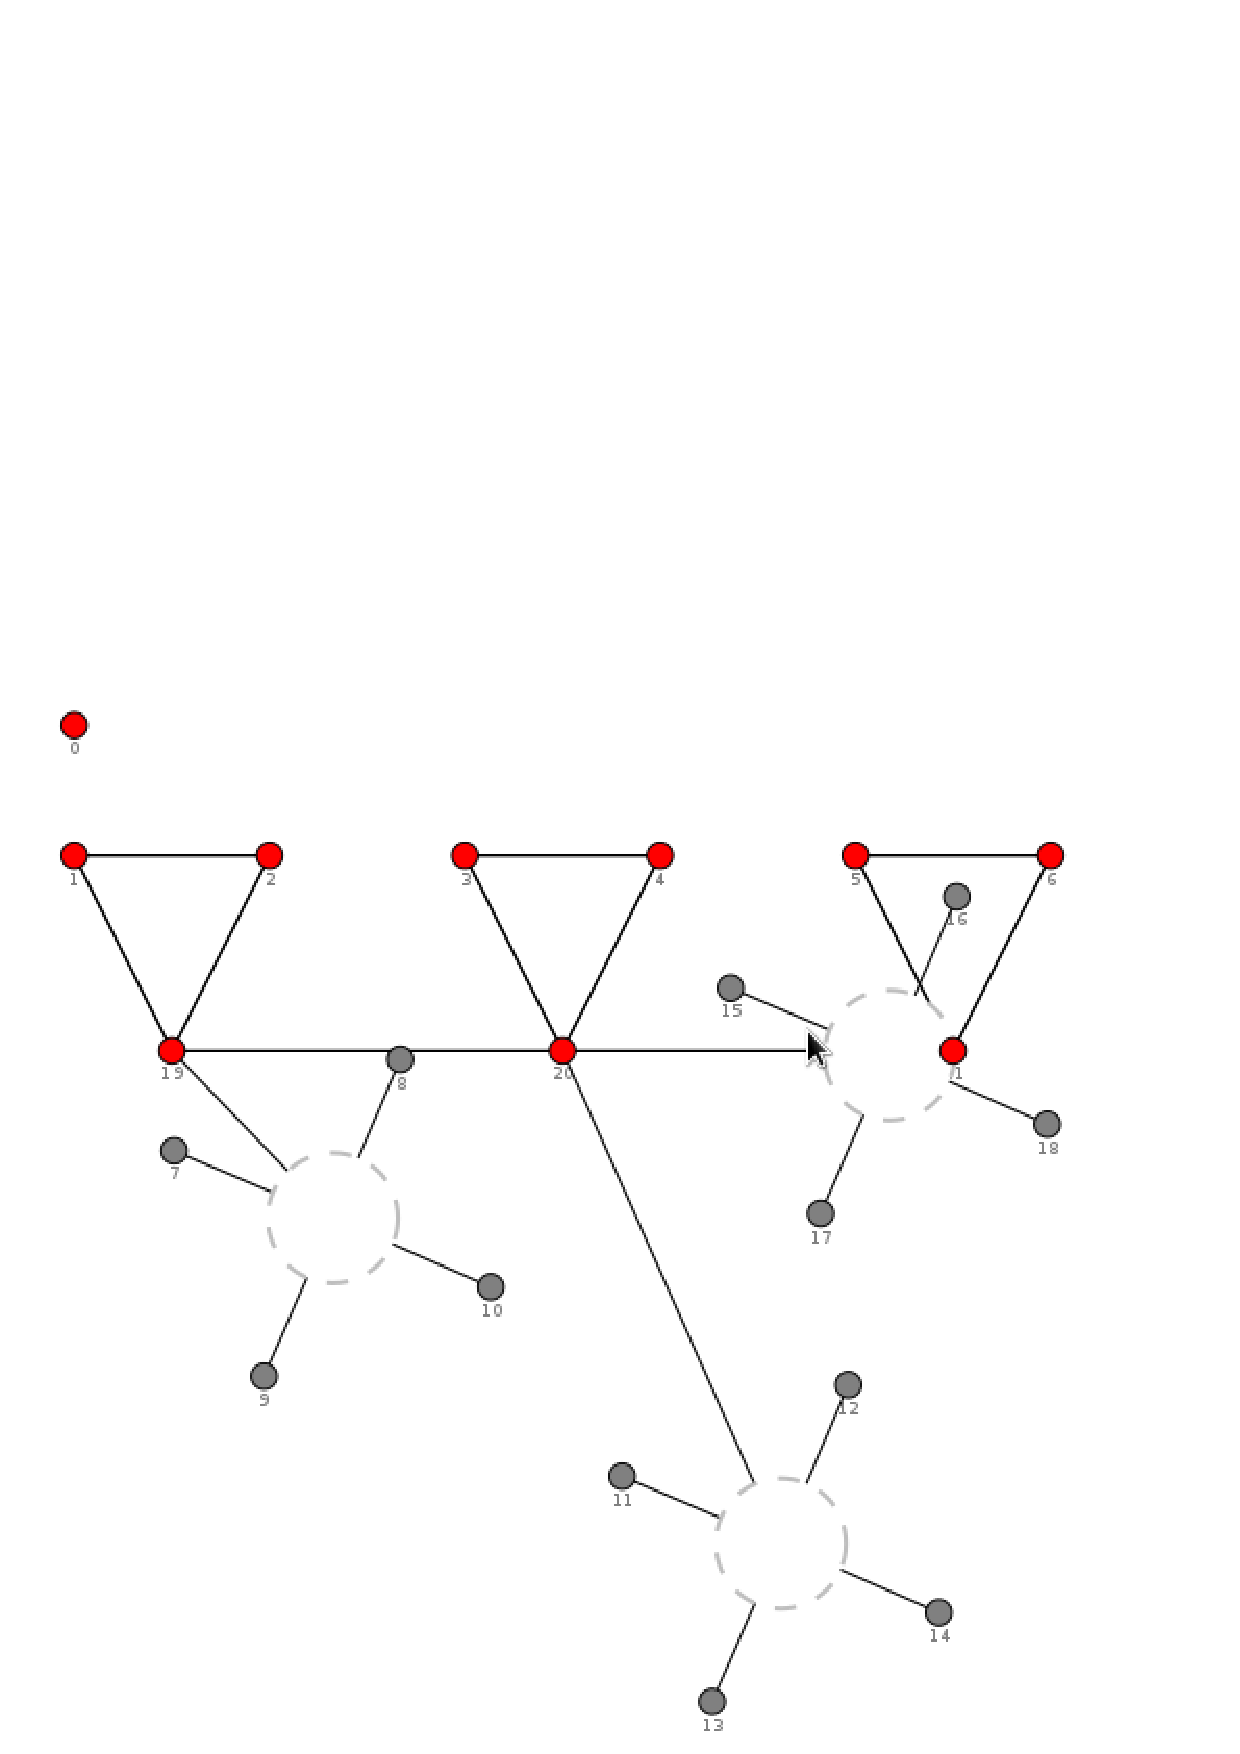
\includegraphics[scale=0.6]{topology.png}}
\caption{Topology for experiments}
\label{fig:exptop}
\end{figure}

\section{Methodology}
To test the success rate of ICN we measure the Satisfied Interest packets and
the Timed Out Interest packets to obtain a simple effectiveness metric for the 
network.  
The client node that is picked to create Interests is chosen randomly in every
 simulation execution.



\section{Results}

\begin{figure}[h]
\centering
\resizebox{\columnwidth}{!}{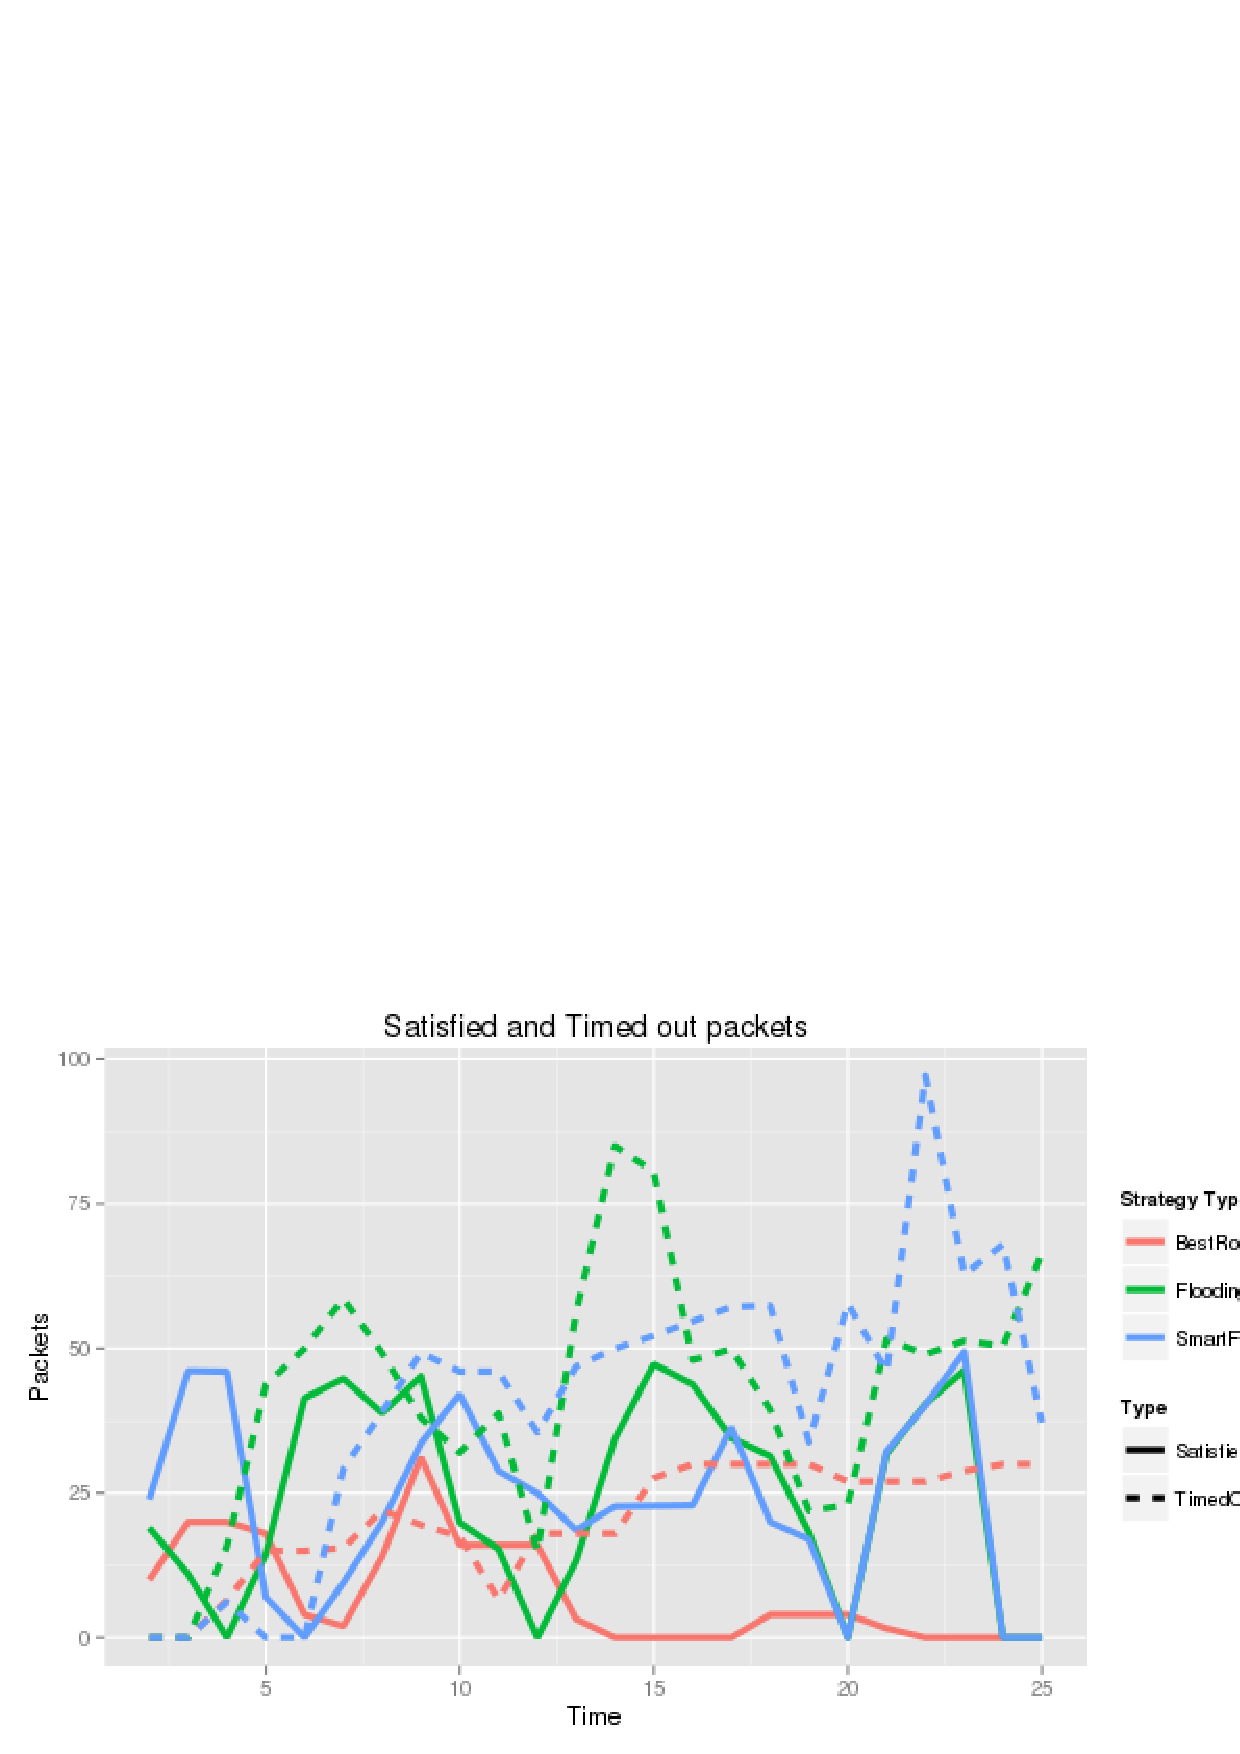
\includegraphics{satisfied-timeout.png}}
\caption{Satisfied and Timed Out Interest Packet}
\label{fig:sattimeint}
\end{figure}


\section{Future work}

\section*{Acknowledgement}
This research was supported by a grant-in-aid from the High-Tech Research
Center Project of the Ministry of Education, Culture, Sports, Science and
Technology (MEXT) \cite{mext:2014:Online}, Japan.

\bibliographystyle{acm}
\bibliography{myrefs}

\end{document}
